\documentclass[11pt]{article}

\usepackage[margin=1in]{geometry}
\usepackage{graphicx}
\usepackage{booktabs}
\usepackage{array}
\usepackage{longtable}
\usepackage{float}
\usepackage{caption}
\usepackage{amsmath}
\usepackage{enumitem}
\usepackage{xcolor}
\usepackage{url}
\usepackage[hidelinks]{hyperref}

\setlist[itemize]{leftmargin=1.4em}
\setlist[enumerate]{leftmargin=1.6em}
\captionsetup{font=small,labelfont=bf}

\newcommand{\code}[1]{\texttt{#1}}
\newcommand{\metric}[1]{\textbf{#1}}

\title{Enhanced Report: MLSS Exoplanet Habitability Classifier}
\author{Bhargav Dave}
\date{\today}

\begin{document}

\maketitle

\begin{abstract}
This enhanced report documents the transformation of a notebook-only graduate MLSS exoplanet habitability classifier into a reproducible, modular, testable tabular machine learning project. The original task predicts a binary \code{habitable?} label from selected Kepler Object of Interest (KOI) features. The enhanced project adds dependency management, configuration, a reusable Python package, a training CLI, leakage-safe scikit-learn pipelines, synthetic-data tests, generated evaluation artifacts, and scientific caveats. Newly computed enhanced-pipeline results show that Logistic Regression with Elastic Net regularization and RBF SVM tie for the best test macro F1 score at 0.9648, while XGBoost has the best cross-validated macro F1 score at 0.9559, closely followed by Random Forest at 0.9557. These high scores should be interpreted as performance on a supplied derived label-list distinction, not proof of biological habitability.
\end{abstract}

\tableofcontents
\newpage

\section{Project Motivation}

Exoplanet habitability classification is an appealing machine learning problem because it connects tabular predictive modeling with a scientifically meaningful question: which observed planet candidates resemble previously labeled habitable candidates? The project is also a useful graduate-level data science exercise because it includes messy provenance, class imbalance, feature selection, model comparison, and interpretability concerns.

The scientific framing needs care. This project does not detect life, measure atmospheric habitability, or prove surface conditions. It predicts a binary label, \code{habitable?}, derived from supplied habitable and non-habitable lists. The resulting models should therefore be read as classifiers of an existing label-list distinction rather than as definitive physical habitability models.

\section{Dataset and Provenance}

The original notebook frames the data as Kepler Object of Interest (KOI) / Kepler cumulative exoplanet data combined with separate habitable and non-habitable planet lists. The enhanced repository expects three local raw Excel files:

\begin{itemize}
  \item \code{data/raw/cumulative-exoplanets.xlsx}
  \item \code{data/raw/habitable\_planets\_detailed\_list.xlsx}
  \item \code{data/raw/non\_habitable\_planets\_confirmed\_detailed\_list.xlsx}
\end{itemize}

Raw data is intentionally not committed to GitHub. During validation, the raw files were copied from the parent/original project folder into ignored local \code{data/raw/}. They remained ignored and were not staged.

The exact provenance and version of the three local Excel files remain uncertain unless visible from the files themselves. The NASA Exoplanet Archive provides external documentation for KOI table columns and is used here as column-definition context, not as a claim that the local Excel files were downloaded directly from a specific archive endpoint in this exact form \cite{nasaKoiColumns}.

\section{Original Notebook Workflow}

The original notebook is preserved at \code{notebooks/mlss-dacss756-final-project-bdave\_v10.ipynb}. Its title currently says ``Predicting the Hability of Exoplanets using Machine Learning''; the typo should eventually be corrected to ``Habitability,'' but the notebook itself remains unchanged.

The historical notebook workflow:

\begin{enumerate}
  \item Load the cumulative KOI-style table and the two label-list files.
  \item Start from a cumulative table visible in the notebook as 9,564 rows and 141 columns.
  \item Keep \code{kepoi\_name} and 15 numeric KOI features.
  \item Construct \code{habitable?} by assigning 1 to the habitable list and 0 to the non-habitable list.
  \item Merge the labels onto selected KOI features by \code{kepoi\_name}.
  \item Produce a modeling dataset visible in the notebook as 2,372 rows and 17 columns.
  \item Remove outliers from \code{koi\_smass} using IQR multiplier 1.5 and from \code{koi\_prad} using IQR multiplier 2.0, leaving 2,121 rows.
  \item Use an 80/20 stratified train-test split with \code{random\_state=42}.
  \item Use median imputation.
  \item Compare Logistic Regression variants, Random Forest, Gradient Boosting, XGBoost, and SVM variants using macro F1.
\end{enumerate}

\section{Feature Space}

The model uses 15 numeric features, listed in Table~\ref{tab:features}. These include planet-candidate quantities, orbital quantities, and host-star quantities.

\begin{longtable}{>{\ttfamily}p{0.22\textwidth}p{0.70\textwidth}}
\caption{Selected KOI features used by the project.}
\label{tab:features}\\
\toprule
\normalfont Feature & Description \\
\midrule
\endfirsthead
\toprule
\normalfont Feature & Description \\
\midrule
\endhead
koi\_period & Orbital period, usually in days. \\
koi\_ror & Planet-star radius ratio. \\
koi\_srho & Fitted stellar density associated with the transit model. \\
koi\_prad & Planetary radius in Earth radii. \\
koi\_sma & Semi-major axis in astronomical units. \\
koi\_teq & Estimated equilibrium temperature in Kelvin. \\
koi\_insol & Insolation flux relative to Earth. \\
koi\_dor & Planet-star distance divided by stellar radius. \\
koi\_count & Count of planets or KOIs associated with the system in the KOI table context. \\
koi\_steff & Stellar effective temperature in Kelvin. \\
koi\_slogg & Stellar surface gravity, typically in $\log_{10}(\mathrm{cm}/\mathrm{s}^2)$. \\
koi\_smet & Stellar metallicity in dex. \\
koi\_srad & Stellar radius in solar radii. \\
koi\_smass & Stellar mass in solar masses. \\
koi\_eccen & Orbital eccentricity. \\
\bottomrule
\end{longtable}

\section{Target Construction and Scientific Caveat}

The target variable \code{habitable?} is a derived supervised label. The notebook assigns:

\begin{itemize}
  \item \code{1} to rows in the supplied habitable planet list.
  \item \code{0} to rows in the supplied non-habitable confirmed planet list.
\end{itemize}

Those labels are merged onto selected KOI features by \code{kepoi\_name}. This design is suitable for supervised learning, but it does not create a direct biological outcome. If the supplied label lists were created using variables similar to the predictors, then the model may learn the label-generation logic. This is possible target leakage in the scientific sense, even if the machine learning pipeline itself is engineered to avoid train/test preprocessing leakage.

\section{Enhanced Project Architecture}

The enhanced repository now separates project concerns:

\begin{itemize}
  \item \code{README.md}: setup, usage, caveats, and project overview.
  \item \code{requirements.txt}: lightweight dependency management.
  \item \code{configs/default.yaml}: paths, features, target, split settings, outlier rules, scoring, and model grids.
  \item \code{src/exoplanet\_classifier/}: reusable Python package.
  \item \code{scripts/train.py}: command-line training entrypoint.
  \item \code{docs/}: data provenance and scientific caveats.
  \item \code{tests/}: synthetic-data pytest tests.
  \item \code{reports/}: generated model reports and explanatory report packages.
  \item \code{figures/}: generated evaluation figures.
\end{itemize}

The project also keeps raw data, model artifacts, generated zip files, caches, and local Codex reports ignored by Git.

\section{Config-Driven Workflow}

The file \code{configs/default.yaml} defines the workflow instead of burying parameters in notebook cells. It specifies:

\begin{itemize}
  \item Raw data paths under \code{data/raw/}.
  \item ID column: \code{kepoi\_name}.
  \item Target column: \code{habitable?}.
  \item The 15 feature names.
  \item Test size: 0.2.
  \item Random seed: 42.
  \item Cross-validation folds: 5.
  \item Main scoring metric: \code{f1\_macro}.
  \item Outlier rules: \code{koi\_smass: 1.5} and \code{koi\_prad: 2.0}.
  \item Bounded grids for DummyClassifier, Logistic Elastic Net, SVM RBF, Random Forest, Gradient Boosting, and XGBoost.
\end{itemize}

This makes the workflow easier to inspect, reproduce, and adjust without rewriting project code.

\section{Data Pipeline}

The enhanced data pipeline:

\begin{enumerate}
  \item Checks that the three expected raw files exist.
  \item Loads Excel files using pandas and openpyxl.
  \item Selects \code{kepoi\_name} plus the configured feature columns.
  \item Constructs the binary \code{habitable?} label from the two label-list files.
  \item Merges labels and features by \code{kepoi\_name}.
  \item Applies the configured IQR outlier rules.
  \item Splits the cleaned table into \code{X} and \code{y}.
  \item Creates a stratified train-test split with \code{random\_state=42}.
\end{enumerate}

The full run confirmed the expected processed shape:

\begin{itemize}
  \item Prepared dataset rows after configured cleaning: 2,121.
  \item Training rows: 1,696.
  \item Test rows: 425.
\end{itemize}

\section{Leakage-Safe Preprocessing}

The enhanced workflow uses scikit-learn \code{Pipeline} and \code{ColumnTransformer} patterns \cite{sklearnPipeline,sklearnColumnTransformer}. Median imputation is inside the model pipeline, not fit globally before cross-validation. Scaling is inside the pipeline for Logistic Regression and SVM, while tree-based models use median imputation without scaling.

This matters because preprocessing should be learned only from the training fold inside each cross-validation split. The model-selection step uses \code{GridSearchCV} with \code{StratifiedKFold}, so preprocessing and model fitting are evaluated together within each fold \cite{sklearnCrossValidation,sklearnGridSearchCV}.

\section{Model Registry and Training CLI}

The project includes a model registry for:

\begin{itemize}
  \item DummyClassifier baseline.
  \item Logistic Regression with Elastic Net regularization.
  \item RBF SVM.
  \item Random Forest.
  \item Gradient Boosting.
  \item XGBoost, when installed.
\end{itemize}

The training CLI is:

\begin{center}
\code{python scripts/train.py --config configs/default.yaml --model all}
\end{center}

It also supports \code{--model} for individual models and \code{--smoke-test} for lightweight validation. XGBoost was installed and ran successfully in the validation step. XGBoost is a scalable tree boosting system described by Chen and Guestrin and documented by the XGBoost project \cite{chenGuestrin2016XGBoost,xgboostDocs}.

\section{Testing and Validation}

The enhanced validation step confirmed:

\begin{itemize}
  \item Dependencies installed successfully with \code{python -m pip install -r requirements.txt}.
  \item Python version: 3.10.5.
  \item Core imports passed for \code{numpy}, \code{pandas}, \code{sklearn}, \code{yaml}, \code{matplotlib}, and \code{pytest}.
  \item XGBoost was available and ran successfully.
  \item Tests passed: 7 passed in 21.13 seconds.
  \item Raw files were copied from the parent/original project folder into ignored local \code{data/raw/}.
  \item Raw files remained ignored and were not staged.
  \item Smoke training succeeded.
  \item Full bounded training succeeded.
  \item No model grids were changed during the run.
\end{itemize}

\section{Historical Notebook Results}

Table~\ref{tab:historical-results} shows historical notebook results. These are included for comparison only and were not regenerated by rerunning the notebook.

\begin{table}[H]
\centering
\caption{Historical notebook model comparison.}
\label{tab:historical-results}
\small
\begin{tabular}{lcc}
\toprule
Model & Historical CV macro F1 & Historical test macro F1 \\
\midrule
Logistic Regression Elastic Net & 0.9419 & 0.9648 \\
Random Forest & 0.9718 & 0.9540 \\
Gradient Boosting / ``Random Forest With GBM'' & 0.9720 & 0.9540 \\
XGBoost & 0.9647 & 0.9413 \\
SVM RBF & 0.9421 & 0.9648 \\
\bottomrule
\end{tabular}
\end{table}

\section{Enhanced Pipeline Results}

Table~\ref{tab:enhanced-results} shows newly computed enhanced-pipeline results from \code{reports/model\_comparison.csv}. These metrics were generated by the modular training pipeline.

\begin{table}[H]
\centering
\caption{Newly computed enhanced-pipeline model comparison.}
\label{tab:enhanced-results}
\small
\begin{tabular}{lrrrrrrr}
\toprule
Model & CV F1 & Acc. & Prec. & Recall & Test F1 & ROC-AUC & PR-AUC \\
\midrule
Logistic Elastic Net & 0.9327 & 0.9929 & 0.9553 & 0.9748 & 0.9648 & 0.9990 & 0.9809 \\
SVM RBF & 0.9356 & 0.9929 & 0.9553 & 0.9748 & 0.9648 & 0.9992 & 0.9876 \\
Gradient Boosting & 0.9372 & 0.9906 & 0.9363 & 0.9736 & 0.9540 & 0.9547 & 0.9527 \\
Random Forest & 0.9557 & 0.9906 & 0.9363 & 0.9736 & 0.9540 & 0.9967 & 0.9578 \\
XGBoost & 0.9559 & 0.9882 & 0.9323 & 0.9508 & 0.9413 & 0.9979 & 0.9582 \\
DummyClassifier & 0.4868 & 0.9482 & 0.4741 & 0.5000 & 0.4867 & 0.5000 & 0.0518 \\
\bottomrule
\end{tabular}
\end{table}

\section{Comparative Analysis}

Enhanced test macro F1 reproduces the historical test ranking closely. Logistic Elastic Net and SVM RBF tie for the best enhanced test macro F1 at 0.9648, matching the top historical test score. Random Forest and Gradient Boosting both reach 0.9540, and XGBoost reaches 0.9413, again matching the historical test pattern.

The enhanced CV values are generally lower than the historical notebook CV values. This is plausible because the enhanced workflow uses leakage-safer preprocessing inside scikit-learn pipelines, shuffled \code{StratifiedKFold}, and smaller bounded grids. The enhanced pipeline is designed for reproducibility and auditability rather than exhaustive hyperparameter search.

The DummyClassifier baseline is much worse: test macro F1 = 0.4867, ROC-AUC = 0.5, and PR-AUC = 0.0518. This confirms that the trained models are doing substantially more than majority-class prediction.

XGBoost has the best enhanced CV macro F1 at 0.9559, with Random Forest essentially tied at 0.9557. However, those models do not have the best test macro F1. This difference reinforces that model ranking is not perfectly stable on a small positive test set.

\section{Confusion Matrix and Class-Specific Interpretation}

The test set contains 425 rows, with 22 positive class cases visible in the classification reports. Because the positive class is small, a few predictions can materially change rare-class precision, recall, and F1.

Logistic Elastic Net and SVM RBF both report class 1 precision 0.91, recall 0.95, and F1 0.93 on 22 positive test cases. Random Forest and Gradient Boosting report class 1 precision 0.88, recall 0.95, and F1 0.91. XGBoost reports class 1 precision 0.87, recall 0.91, and F1 0.89. DummyClassifier predicts only the majority class, so class 1 precision, recall, and F1 are all 0.00.

\begin{figure}[H]
  \centering
  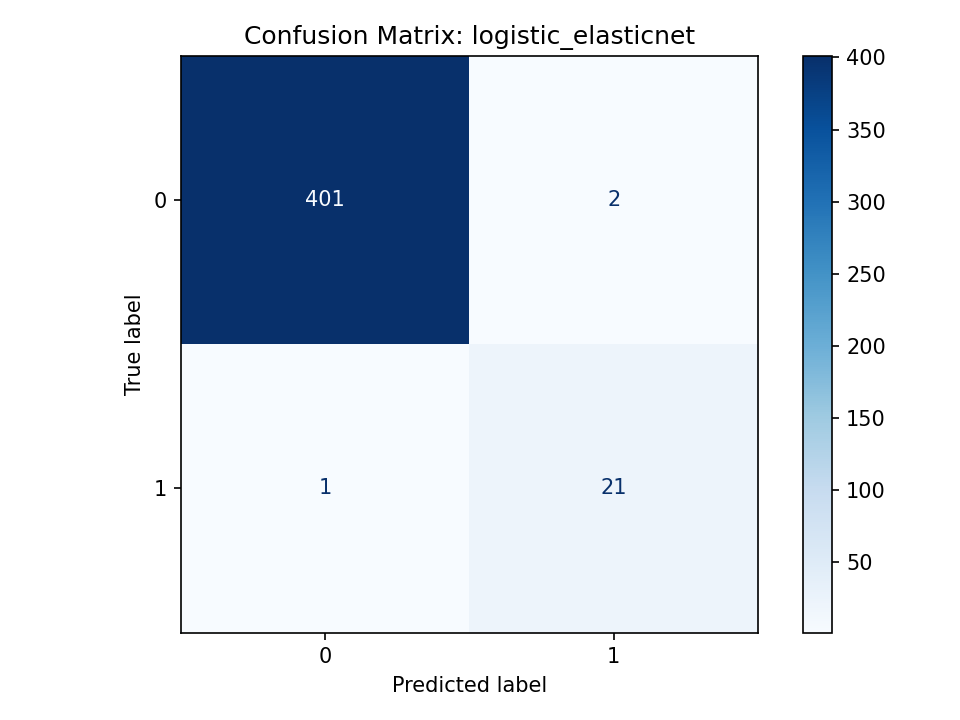
\includegraphics[width=0.48\textwidth]{figures/confusion_matrix_logistic_elasticnet.png}
  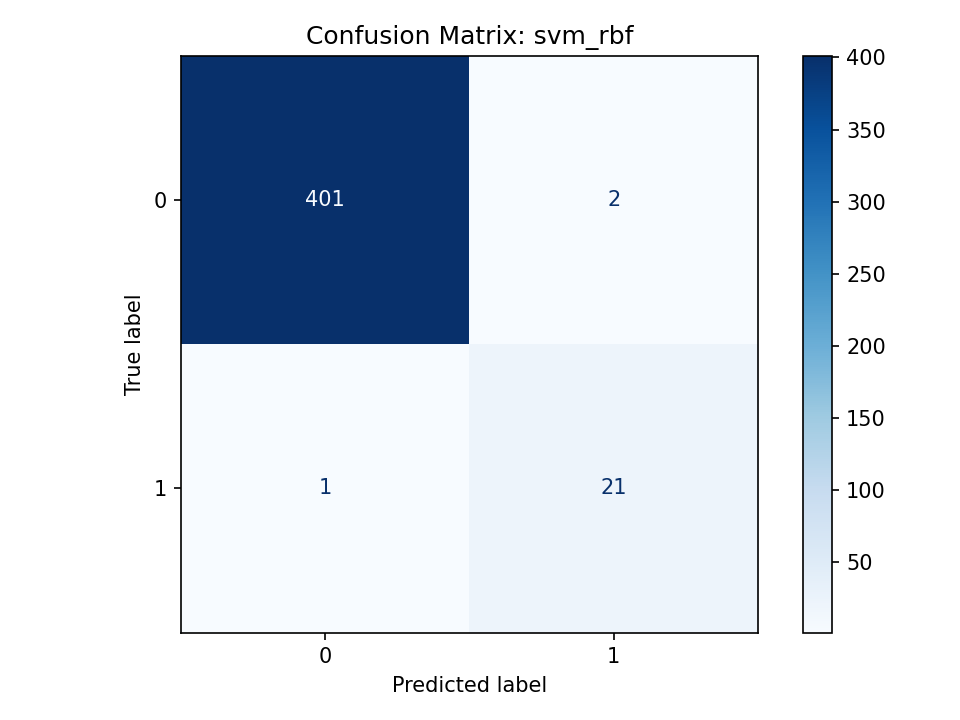
\includegraphics[width=0.48\textwidth]{figures/confusion_matrix_svm_rbf.png}
  \caption{Confusion matrices for the two models tied for best enhanced test macro F1: Logistic Elastic Net and SVM RBF.}
  \label{fig:cm-top}
\end{figure}

\begin{figure}[H]
  \centering
  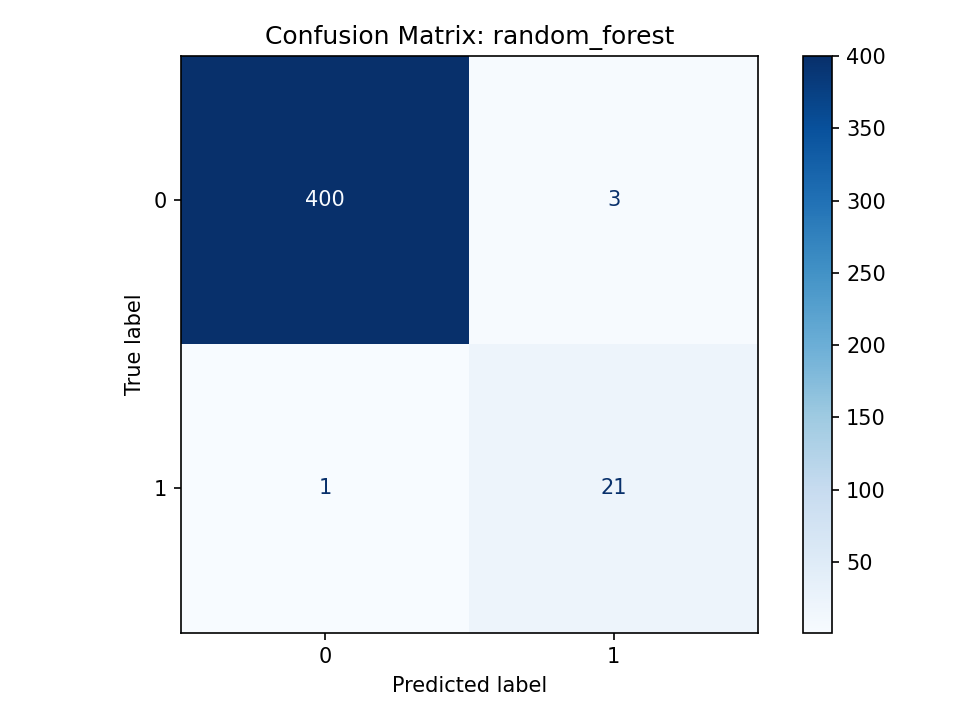
\includegraphics[width=0.48\textwidth]{figures/confusion_matrix_random_forest.png}
  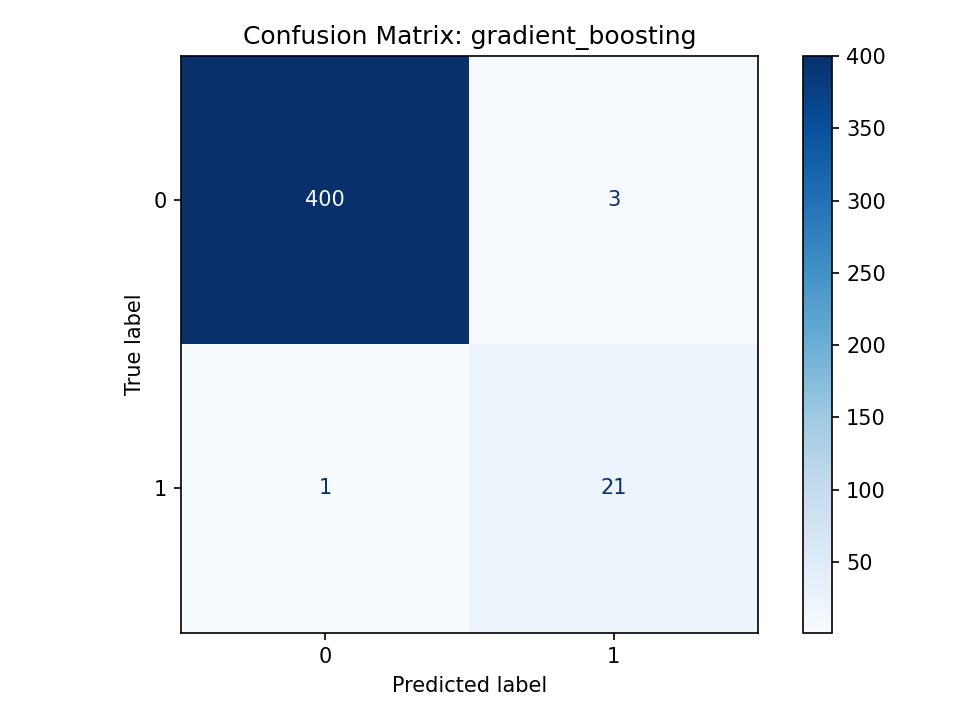
\includegraphics[width=0.48\textwidth]{figures/confusion_matrix_gradient_boosting.png}
  \caption{Confusion matrices for Random Forest and Gradient Boosting.}
  \label{fig:cm-trees}
\end{figure}

\begin{figure}[H]
  \centering
  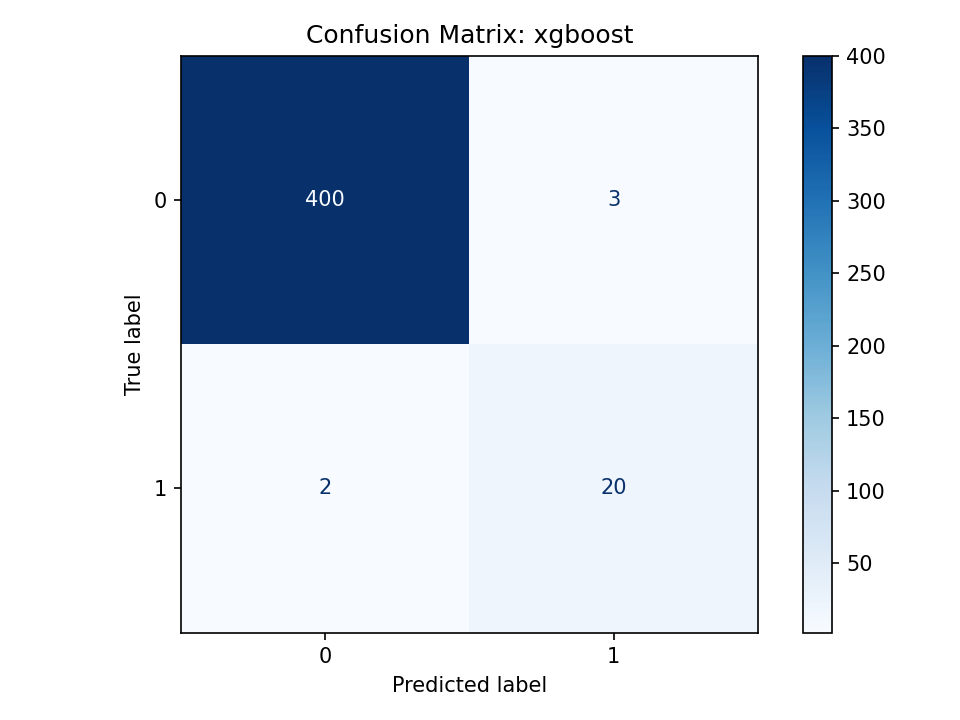
\includegraphics[width=0.48\textwidth]{figures/confusion_matrix_xgboost.png}
  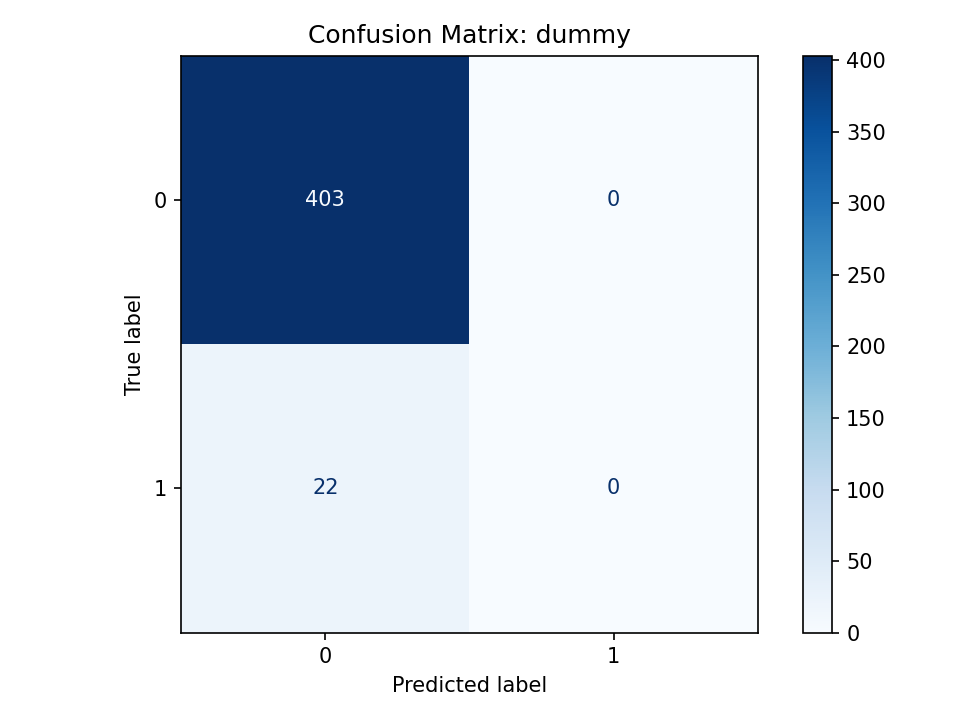
\includegraphics[width=0.48\textwidth]{figures/confusion_matrix_dummy.png}
  \caption{Confusion matrices for XGBoost and DummyClassifier. The baseline fails to identify the rare positive class.}
  \label{fig:cm-xgb-dummy}
\end{figure}

\section{ROC, Precision-Recall, and Permutation Importance}

ROC-AUC is high for the trained models, but ROC curves can look optimistic under strong class imbalance. PR-AUC is especially useful here because it focuses more directly on positive-class retrieval under rare-positive conditions.

\begin{figure}[H]
  \centering
  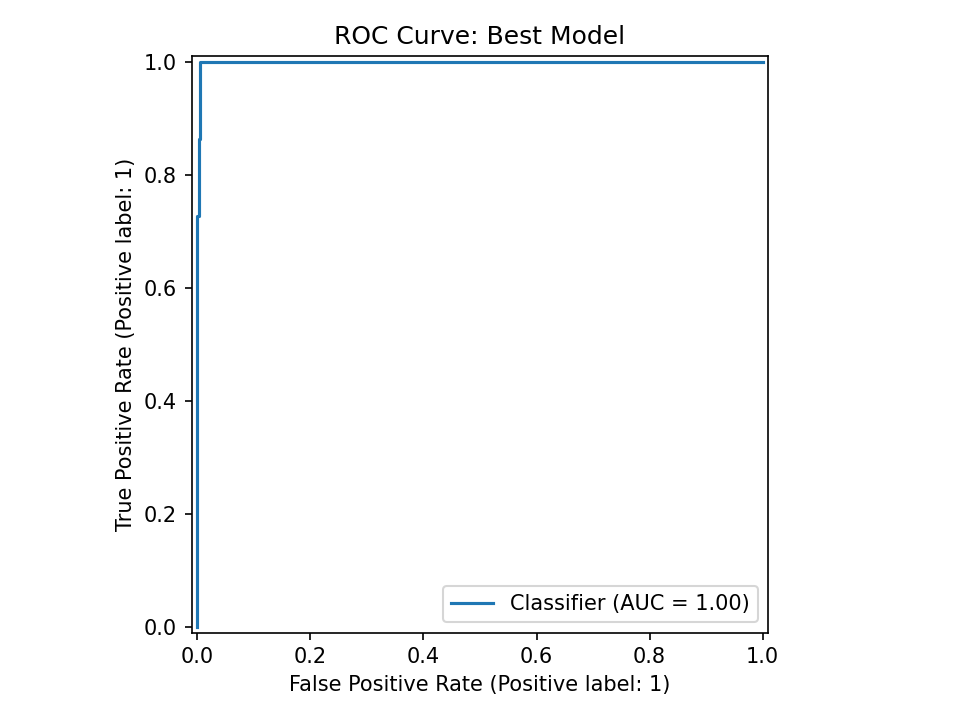
\includegraphics[width=0.78\textwidth]{figures/roc_curve.png}
  \caption{ROC curve for the best model selected by the enhanced training script.}
  \label{fig:roc}
\end{figure}

\begin{figure}[H]
  \centering
  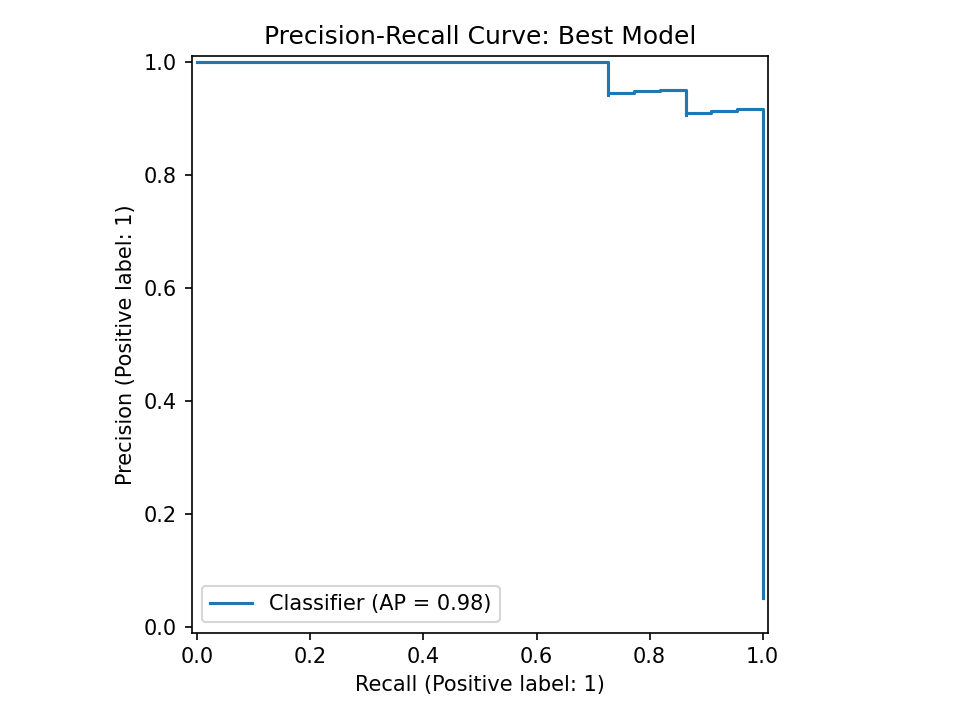
\includegraphics[width=0.78\textwidth]{figures/precision_recall_curve.png}
  \caption{Precision-recall curve for the best model selected by the enhanced training script. PR-AUC is important because the positive class is rare.}
  \label{fig:pr}
\end{figure}

\begin{figure}[H]
  \centering
  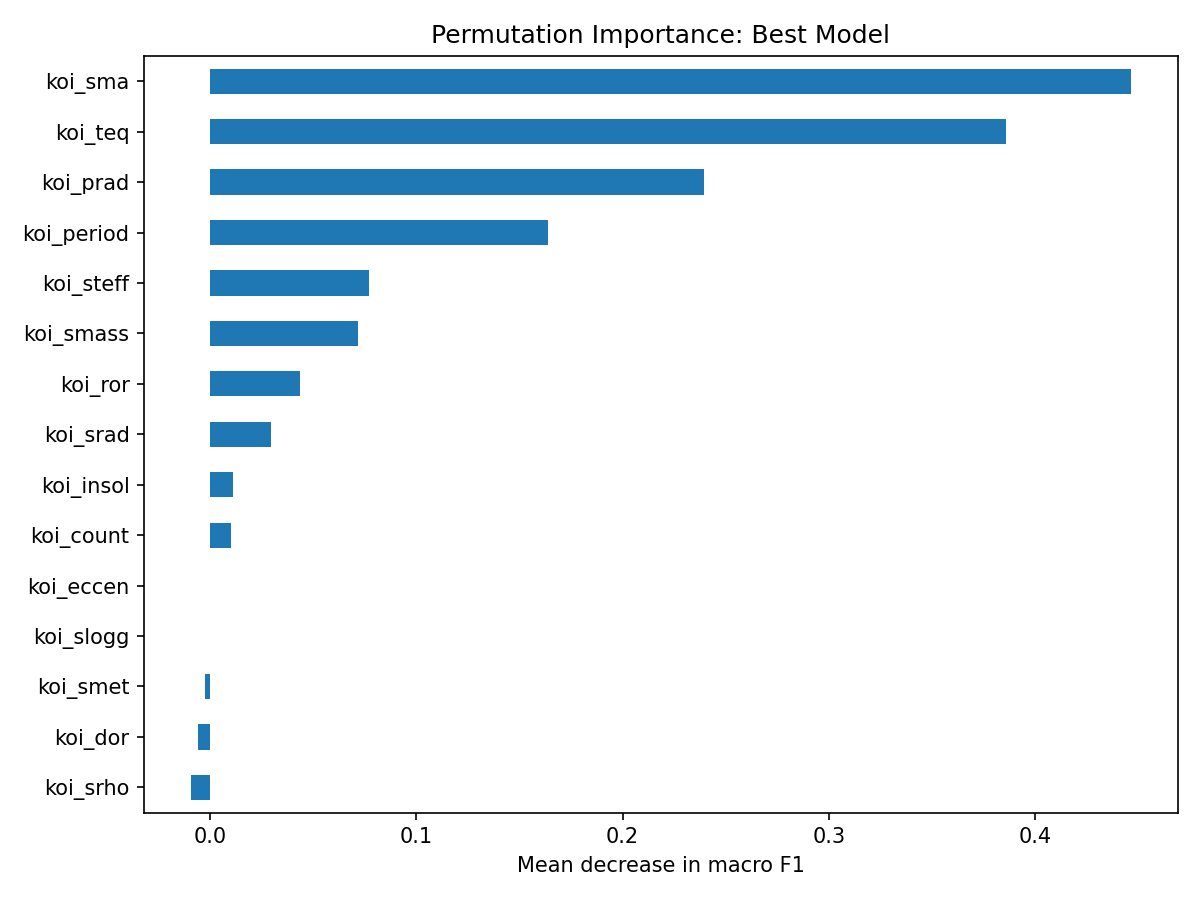
\includegraphics[width=0.80\textwidth]{figures/permutation_importance.png}
  \caption{Permutation importance for the best model. Importance should be interpreted cautiously because features may be correlated and the target label itself is derived.}
  \label{fig:permutation}
\end{figure}

\section{Evaluation Design}

The enhanced pipeline reports several metrics \cite{sklearnF1Score}:

\begin{itemize}
  \item Accuracy: overall fraction of correct predictions.
  \item Macro precision: average precision across classes.
  \item Macro recall: average recall across classes.
  \item Macro F1: average class-level F1 across classes.
  \item Confusion matrix: raw counts of correct and incorrect predictions by class.
  \item ROC-AUC: ranking quality across thresholds.
  \item PR-AUC: precision-recall tradeoff, especially informative for rare positive classes.
\end{itemize}

Macro F1 remains the main metric because the class distribution is highly imbalanced. Accuracy alone is misleading: the dummy baseline reaches 0.9482 accuracy by predicting the majority class, yet its macro F1 is only 0.4867 and its class 1 F1 is 0.00.

\section{Software Engineering Improvements}

The enhancement is primarily an engineering and reproducibility upgrade:

\begin{itemize}
  \item Modular code replaces notebook-only logic.
  \item Configuration separates paths, features, split settings, model grids, and outputs.
  \item Tests validate imports, config loading, feature lists, preprocessing, model registry, and tiny model training.
  \item The training script can run smoke tests or full bounded searches.
  \item Raw data and generated artifacts are handled with explicit Git hygiene.
  \item Scientific caveats and data provenance are documented.
  \item Overleaf-ready reporting is separated from code execution.
\end{itemize}

\section{Limitations}

Important limitations remain:

\begin{itemize}
  \item The target is a derived label, not a direct biological habitability measurement.
  \item The positive class is small and imbalanced.
  \item Test performance depends on only 22 positive examples.
  \item Possible label leakage exists if the label lists were created from variables similar to the predictors.
  \item Exoplanet measurements have uncertainty, but the pipeline uses point estimates.
  \item Exoplanet catalogs contain discovery and selection biases.
  \item The exact provenance/version of the local raw Excel files remains uncertain.
  \item There is no CI pipeline yet.
  \item There is no model card yet.
  \item Threshold tuning and calibration were not performed.
\end{itemize}

Most importantly, strong predictive performance may mean that the model successfully reproduces the supplied label-list distinction. It should not be presented as proof of actual planetary habitability.

\section{Future Work}

Recommended next steps:

\begin{itemize}
  \item Add a verified data acquisition script if licensing and source access permit.
  \item Define the scientific label more rigorously.
  \item Add uncertainty-aware modeling or sensitivity analysis.
  \item Add a model card and data card.
  \item Add continuous integration for tests.
  \item Add optional experiment tracking only if it stays lightweight.
  \item Add threshold tuning and probability calibration.
  \item Use repeated cross-validation or bootstrap analysis to assess ranking stability.
  \item Add a small dashboard only if it supports interpretation rather than decoration.
\end{itemize}

\newpage
\bibliographystyle{plain}
\bibliography{references}

\end{document}
